% Created 2021-09-11 Sat 16:41
% Intended LaTeX compiler: xelatex
\documentclass[letterpaper]{article}
\usepackage{graphicx}
\usepackage{grffile}
\usepackage{longtable}
\usepackage{wrapfig}
\usepackage{rotating}
\usepackage[normalem]{ulem}
\usepackage{amsmath}
\usepackage{textcomp}
\usepackage{amssymb}
\usepackage{capt-of}
\usepackage{hyperref}
\usepackage[margin=1in]{geometry}
\usepackage{fontspec}
\usepackage{indentfirst}
\setmainfont[ItalicFont = LiberationSans-Italic, BoldFont = LiberationSans-Bold, BoldItalicFont = LiberationSans-BoldItalic]{LiberationSans}
\newfontfamily\NHLight[ItalicFont = LiberationSansNarrow-Italic, BoldFont       = LiberationSansNarrow-Bold, BoldItalicFont = LiberationSansNarrow-BoldItalic]{LiberationSansNarrow}
\newcommand\textrmlf[1]{{\NHLight#1}}
\newcommand\textitlf[1]{{\NHLight\itshape#1}}
\let\textbflf\textrm
\newcommand\textulf[1]{{\NHLight\bfseries#1}}
\newcommand\textuitlf[1]{{\NHLight\bfseries\itshape#1}}
\usepackage{fancyhdr}
\pagestyle{fancy}
\usepackage{titlesec}
\usepackage{titling}
\makeatletter
\lhead{\textbf{\@title}}
\makeatother
\rhead{\textrmlf{Compiled} \today}
\lfoot{\theauthor\ \textbullet \ \textbf{2021-2022}}
\cfoot{}
\rfoot{\textrmlf{Page} \thepage}
\titleformat{\section} {\Large} {\textrmlf{\thesection} {|}} {0.3em} {\textbf}
\titleformat{\subsection} {\large} {\textrmlf{\thesubsection} {|}} {0.2em} {\textbf}
\titleformat{\subsubsection} {\large} {\textrmlf{\thesubsubsection} {|}} {0.1em} {\textbf}
\setlength{\parskip}{0.45em}
\renewcommand\maketitle{}
\author{Houjun Liu}
\date{\today}
\title{Object Electrostatic Polarization}
\hypersetup{
 pdfauthor={Houjun Liu},
 pdftitle={Object Electrostatic Polarization},
 pdfkeywords={},
 pdfsubject={},
 pdfcreator={Emacs 27.2 (Org mode 9.4.4)}, 
 pdflang={English}}
\begin{document}

\maketitle


\section{The Rods and Paper Experiment}
\label{sec:org58df31a}
\begin{figure}[htbp]
\centering
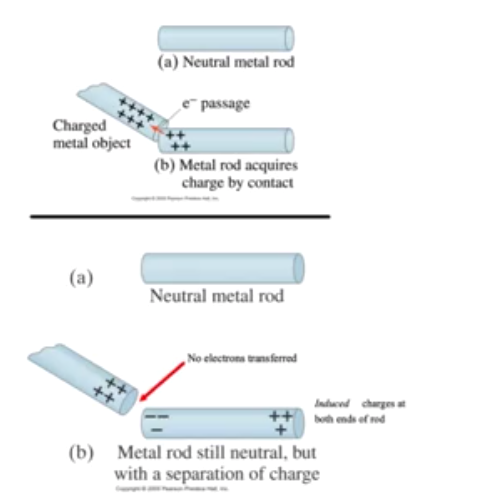
\includegraphics[width=.9\linewidth]{./2020PHYS201/Screen Shot 2020-08-24 at 4.46.46 PM.png}
\caption{Screen Shot 2020-08-24 at 4.46.46 PM.png}
\end{figure}

\textbf{Scenario 1}

\begin{itemize}
\item Taking neutral rod + close, positively charged, rod

\begin{itemize}
\item Electrons will move from the neutral rod to the charged rod
\item Balances the charge out
\end{itemize}
\end{itemize}

\textbf{Scenario 2}

\begin{itemize}
\item Taking neutral rod + slightly farther, positively charged, rod

\begin{itemize}
\item The neutral rod "polarizes", repelling the positively charged
protons off to one side while attracting all the electrons towards
it
\item There is a net force of attraction to the "left" on the example
image --- towards the charged rod
\end{itemize}
\end{itemize}

Recall that per the
physics\href{KBhPHYS201D1AtHomeActivity.org}{KBhPHYS201D1AtHomeActivity}
D1 At home Activity, pieces of paper sometime flow towards the charged
rod, then back again. Why?

About how that works\ldots{}

\begin{enumerate}
\item The charged rod polarizes the paper
\item The paper's newfound positive end attract with the plastic rod's
negative end
\item The paper has a net positive force towards the rod, so it accelerates
towards it
\item Electrons, once connected, tries to flow back onto the paper
\item The paper neutralizes, then falls to the ground
\item Repeat from (1)
\end{enumerate}
\end{document}
